\chapter{MEF parte II}

\textbf{Definición: }Sea $M=\{S,I,D,f,g,s^*\}$ una MEF.

\begin{enumerate}
\item Para $s_i,s_j\in S$ se dice que $s_j$ es \textbf{alcanzable} desde $s_i$ si $s_i=s_j$ o si hay cadenas de entrada $w\in I^+$ tal que $f(s_i,w)=s$.
\item Un estado $s\in S$ se dice \textbf{transitorio} si $f(s,w)=s$ para $w\in I^* \Rightarrow w=\varepsilon$, es decir, no hay $w\in I^+ /f(s,w)=s$.


\textbf{Ejemplo: }Sea la MEF con diagrama de transición(Figura \ref{img_8_1}).

%imagen
\begin{figure}[h!]
\centering
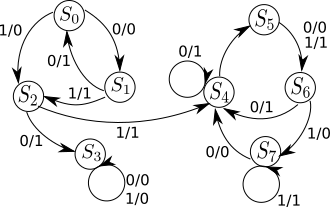
\includegraphics[width=0.35\textwidth]{img_8_1.png}
\caption{Diagrama de Transición}\label{img_8_1}
\end{figure}

\begin{itemize}
\item ¿ Desde qué estados es alcanzable $s_3$?
	
	$s_0,s_1,s_2$
\item ¿ Desde qué estados no es alcanzable $s_3$?

	$s_4,s_5,s_6,s_7$
\item Encuentre un estado transitorio en M.

	$s_2$ es un estado transitorio.
\end{itemize}

\item Un estado $s\in S$ es un estado \textbf{sumidero} si: $f(s,w)=s\qquad \forall w\in I^*$

\item Sea $S_1\in S, \quad I_1 \subseteq I$. Si $ f_1=f|_{S_1\times I_1}$

	$f_1:S_1\times I_1\rightarrow S$ tiene su rango dentro de $S_1$ entonces $g_1=g|_{S_1\times I_1}$
	
	$g_1: S_1\times I_1 \rightarrow O$, entonces $M_1=(S_1,I_1,O_1,f_1,g_1,s^*)$ se llama \textbf{submáquina} de la MEF $M$.
	
\item Una máquina se denomina \textbf{fuertemente conexa} si para cualquier estado $s_i$, $s_j$ es accesible desde $s_i$.

\textbf{Ejemplo: }Usando la MEF anterior.

\begin{itemize}
\item Identifique un estado sumidero.

	$s_3$
\item Encuentre una submáquina.
\begin{itemize}
	\item Sea $s_1=\{s_0,s_1,s_2\}\subseteq S$ y $I_1=\{0,1\}\subseteq I$, 
	$f_1$ tiene algunos estados que caen fuera de $S_1$. ( \xmark )
	
	\item Sea $S_1=\{s_4,s_5,s_6,s_7\}\subseteq S$ y $I=\{0,1\}$ luego $M_1=(S_1,I_1,O,f_1,g_1,s^*)$ es una submáquina de $M$. ( \cmark )
	\item Encuentre una máquina fuertemente conexa.
	
	$M$ no es fuertemente conexa, sin embargo, $M_1$ si es fuertemente conexa.
	
\end{itemize}
\end{itemize}
	

\end{enumerate}

\textbf{Definición: }Para una MEF $M=\{S,I,O,f,g,s^*)$. Sean $s_i,s_j \in S$ dos estados distintos. Una cadena de entrada $w\in I^+$ es llamada \textbf{secuencia de transferencia o transición} desde $s_i$ a $s_j$ si:
\begin{itemize}
\item $f(s_i,w)=s_j$
\item $v\in I^+$ con $f(s_i,v)=s_j\Rightarrow |v|\geq |w|$
\end{itemize}

\textbf{Ejemplo: }Obtener una secuencia de transferencia desde el estado $S_0$ hacia el estado $S_2$ para la MEF $M$ definida sobre $I=\{0,1\}=O$

$S=\{s_0,s_1,s_2,s_3,s_4,s_5,s_6\}$

$M$ está representada por la siguiente tabla.

\begin{center}
$\begin{array}{c|cc|cc}
	&	\multicolumn{2}{c}{f}	&\multicolumn{2}{c}{g}\\
	&0	&1	&0	&1	\\ \hline
s_0	&	s_6		&s_1	&0	&1	\\
s_1	&	s_5		&s_0	&0	&1	\\
s_2	&	s_1		&s_2	&0	&1	\\
s_3	&	s_4		&s_0	&0	&1	\\
s_4	&	s_2		&s_1	&0	&1	\\
s_5	&	s_3		&s_5	&1	&1	\\
s_6	&	s_3		&s_6	&1	&1	\\
\end{array}$
\end{center}

Representamos las transiciones de estado como un árbol(Figura \ref{img_8_2}).

%grafica
\begin{figure}[h!]
\centering
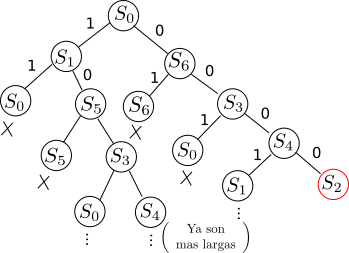
\includegraphics[width=0.4\textwidth]{img_8_2.png}
\caption{Representación como árbol}\label{img_8_2}
\end{figure}

La cadena de transferencia es $w=0000$ con $f(s_0,w)=s_2$ y $g(s_0,w)=0100$. Otra cadena es $v=1000$ pero $|v|>|w|$.

\section{Tipos de MEF}

Para el modelamiento de las calculadoras se ha desarrollado muchos tipos de MEF.

\begin{enumerate}
\item \textbf{Máquina de Moore}
	Una máquina de Moore $M_0=(S,I,O,f,g,s^*)$ es tal que :
\begin{align*}
	S:	&\mbox{ Conjunto de estados}	\\
	I:	&\mbox{ Alfabeto de entrada}	\\
	O:	&\mbox{ Alfabeto de salida}	\\
	f:	&\mbox{ Función de estado siguiente.} f:S\times I\rightarrow S	\\
	g:	&\mbox{ Función de salida, } g:S\rightarrow O	
\end{align*}

\textbf{Representación }\\
\textbf{Ejemplo: }A continuación se presenta la tabla de transición de una máquina de Moore.

\begin{center}
$\begin{array}{c|cc|c}
	&\multicolumn{2}{c|}{f}	&g	\\
S	&a	&b	& 	\\ \hline
s_0	&s_3	&s_2	&0	\\
s_1	&s_1	&s_0	&0	\\
s_2	&s_2	&s_3	&1	\\
s_3	&s_0	&s_1	&0
\end{array}$
\end{center}

Se pide:
\begin{itemize}
\item Dibuje su diagrama de estado.
\item Obtener la cadena de salida para $w=bababbb$
\end{itemize}
\textbf{Solución: }

%grafica
\begin{figure}[h!]
\centering
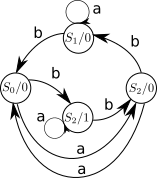
\includegraphics[width=0.2\textwidth]{img_8_3.png}
\caption{Diagrama de Transición}\label{img_8_3}
\end{figure}

\begin{center}
$\begin{array}{c|c|c|c|c|c|c|c}
s_0	&s_2&s_2&s_3&s_0&s_2&s_3&s_1	\\ \hline
b	&a	&b	&a	&b	&b	&b	&		\\ \hline
0	&1	&1	&0	&0	&1	&0	&
\end{array}$
\end{center}

La cadena de salida es $s=0110010$

\item \textbf{Máquina de Mealy: }Fueron estudiados por G.H. Mealy en 1955. En este tipo de máquina las salidas corresponden a transiciones entre estados. Aquí:

\begin{align*}
f:	&S\times I\rightarrow S	\\
g:	&S\times I\rightarrow O
\end{align*}

\textbf{Ejemplo: }Dibuje una máquina de Mealy que imprime el complemento de una cadena de bits de entrada.

\textbf{Solución: }

$S=\{s_0\}$\\
$I=\{0,1\}=O$

\begin{figure}[h!]
\centering
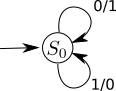
\includegraphics[width=0.15\textwidth]{img_8_4.png}
\caption{Máquina de Mealy}\label{img_8_4}
\end{figure}

\begin{center}
$\begin{array}{c|cc|cc}
	&\multicolumn{2}{c|}{f}	&\multicolumn{2}{c}{g}	\\
	&0	&1	&0	&1	\\ \hline
s_0	&s_0&s_0&1	&0
\end{array}$
\end{center}

\end{enumerate}

\textbf{Teorema: }Si $M_0$ es una máquina de Moore, entonces existe una máquina de Mealy equivalente(Figura \ref{img_8_5}).

\textbf{Método:}
\begin{enumerate}
\item Considere cualquier estado $q_i$ en $M_0$.
\item Suponga que $M_0$ imprime el carácter $t$ al ingresar $q_i$, luego se tiene el rótulo $q_i/t$ en el estado $q_i$.
\item Suponga que hay $n$ arcos de entrada $q_i$ con etiquetas $a_1...a_n$
\item Creamos la máquina de Mealy $M_0$ combinando las etiquetas de los arcos entrantes a $q_i$ a $a_m/t$, $m=1,2,...n$ y cambiamos la etiqueta del estado $q_i/t$ a $q_i$.

%grafico
\begin{figure}[h!]
\centering
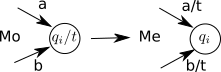
\includegraphics[width=0.30\textwidth]{img_8_5.png}
\caption{Equivalencia entre Mealy y Moore}\label{img_8_5}
\end{figure}
\end{enumerate}
\textbf{Ejemplo: }Convierta la máquina de Moore en la equivalente máquina de Mealy.

%grafico
\begin{figure}[h!]
\centering
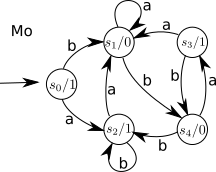
\includegraphics[width=0.25\textwidth]{img_8_6.png}
\caption{Diagrama de Transición}\label{img_8_6}
\end{figure}
%grafico
\begin{figure}[h!]
\centering
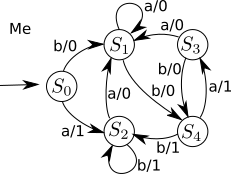
\includegraphics[width=0.25\textwidth]{img_8_7.png}
\caption{Diagrama de Transición}\label{img_8_7}
\end{figure}

\section{MEF sin Salida}
Se usan para el reconocimiento de lenguajes.
\subsection{Autómatas Finitos}

Este tipo de máquinas tienen estados finales y una cadena será reconocida por la máquina si produce una transición desde el estado inicial a una de sus estados finales.

\subsubsection{A.F. Deterministas}
Su salida está limitada a los valores aceptados o rechazados. Formalmente, un $AFD=(S,I,\delta, s^*,F)$
\begin{align*}
	S:	& \mbox{ conjunto finito de estados} (s\not=\phi)	\\
	I:	& \mbox{ alfabeto de entrada}	\\
	\delta:	&\; S\times I\rightarrow S	\\
	F:	& \mbox{ conjunto de estados de aceptacion } (F\subseteq S)	\\
	s^*:	& \mbox{ estado inicial}
\end{align*}

\textbf{Representación: }

Sea el AFD $D$ tal que:
\begin{align*}
S=	&\{s_0,s_1,s_2\}	\\
I=	&\{a,b\}	\\
s^*=	&s_0	\\
F=	&\{s_0\}
\end{align*}
\begin{align*}
\delta(s_0,a)	&=s_1	&\delta(s_0,b)	&=s_2	\\
\delta(s_1,a)	&=s_1	&\delta(s_1,b)	&=s_2	\\
\delta(s_2,a)	&=s_2	&\delta(s_2,b)	&=s_2	
\end{align*}

\textbf{Tabla de Transición: }

\begin{center}
$\begin{array}{c|cc}
	&\multicolumn{2}{c}{\delta}	\\
	&a	&b	\\ \hline
\sharp s_0	&s_1&s_2	\\
s_1	&s_1&s_2	\\
s_2	&s_2&s_2
\end{array}$
\end{center}

\textbf{Diagrama de Transición: }

%grafico
\begin{figure}[h!]
\centering
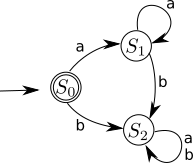
\includegraphics[width=0.25\textwidth]{img_8_8.png}
\caption{Diagrama de Transición de $D$}\label{img_8_8}
\end{figure}

$w=babb$ no es aceptada por $D$.

$F=\{s_1\}$
\begin{figure}[h!]
\centering
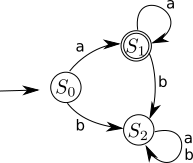
\includegraphics[width=0.25\textwidth]{img_8_9.png}
\caption{Diagrama de Transición}\label{img_8_9}
\end{figure}
\begin{align*}
\left. \begin{array}{c}
	u_1	=a	\\
	u_2	=aa	\\
	\vdots	\\
	u_n	=a^n
	\end{array}\right \} \mbox{Son aceptados por D}
\end{align*}
En el autómata Fig \ref{img_8_9}. Este autómata acepta cadenas formadas solo por $a$. El estado  $s_2$ es un estado \textbf{muerto}.

\textbf{Estado Muerto: }Es aquel estado que no es de aceptación y no parte de él ninguna transición hacia otro estado.

\textbf{Nota: }El AF $D$ se llama determinístico porque el $(s_2)$ estado siguiente queda bien definido (es único) si son conocidos el estado $(s_1)$ y el símbolo $(a)$:
$$\delta(s_1,a) = s_2$$

\section{Autómatas Incompletos}
En algunas ocasiones podemos encontrar autómatas donde no estén definidas todas las transiciones.

Si una cadena hace llegar al AFD a una situación no definida, se asumirá que la cadena no ha sido reconocido por el autómata.
